\section{Introduction }

"AI as a creative tool has improved leaps and bounds since its early incarnations. Generating still images that are interesting, sophisticated and photorealistic is now an easy process that can be done by anybody with an interest, some patience and determination" \cite{scott2024ethics}. The prevalence of AI among the general public has led to extensive dialogue about their ethical implications in producing artwork, or for manufacturing misinformation. One such example of the use of AI is tools like \textit{DALL-E} and \textit{Stable Diffusion}, which generate images from text prompts. In the current digital age, we cannot rely on the transparency of the source of an image, so there exists a need to be able to identify whether an image has been generated by an AI, or a real artist. \Cref{fig:ai_generated_images} shows some examples of AI generated images, which are becoming increasingly difficult to distinguish from real images as the technology improves, underscoring the need for reliable detection methods.

\begin{figure}[h]
    \centering
    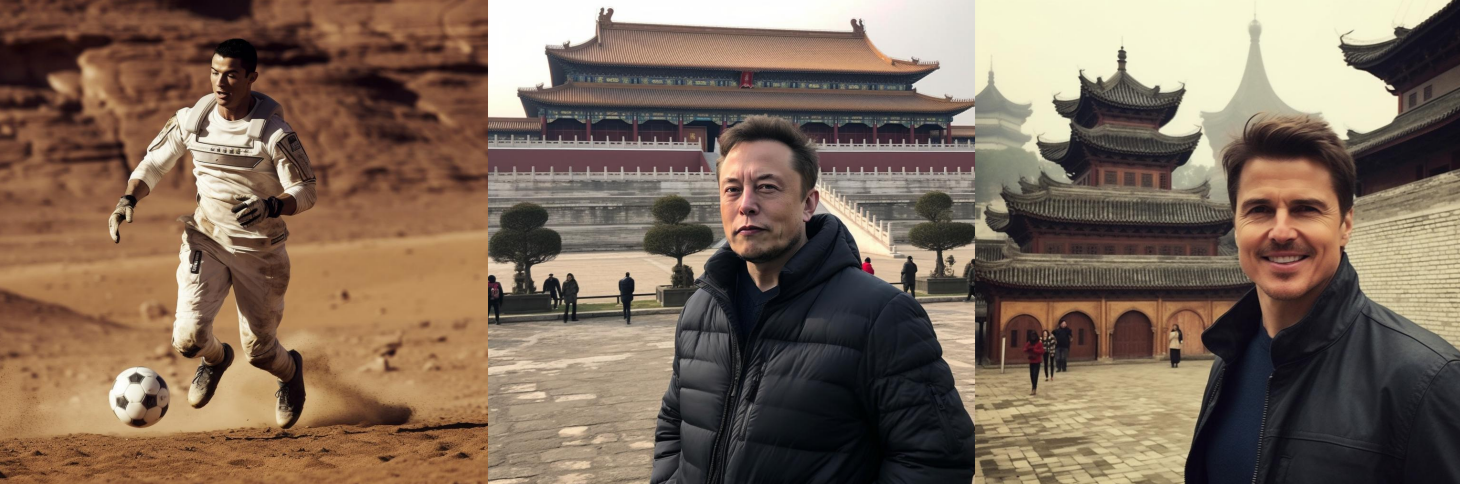
\includegraphics[width=0.8 \linewidth]{figures/ai_generated_images_from_seeing_is_not_believing.png} % Image filename
    \centering
    \caption{AI generated images \cite{lu2023seeingbelievingbenchmarkinghuman}} % Caption
    \label{fig:ai_generated_images} % Label
\end{figure}

\cite{lu2023seeingbelievingbenchmarkinghuman} evaluates both human and AI capabilities in detecting fake images, showing that humans are often deceived by advanced image generation models, while AI-based detection algorithms outperform humans but still misclassify 13\% of images. The study introduction of the Fake2M dataset and new benchmarks (HPBench and MPBench) aims to drive further research and improve the reliability of AI-generated content detection.

\cite{bird2023cifakeimageclassificationexplainable} presents a computer vision approach to distinguishing AI-generated images from real ones, utilising a synthetic dataset created with Latent Diffusion, classification via Convolutional Neural Networks, and interpretability through Grad-CAM. Achieving nearly 93\% accuracy, the study also introduces the CIFAKE dataset, a large collection of real and synthetic images, to support further research on the detection of AI-generated imagery.

It is therefore evident that past research has shown that it is possible to classify images as AI-generated or not, with a high degree of accuracy. This report will explore the process of training a neural network to classify images as either AI-generated or not, and then deploying this model to AWS SageMaker for inference, and evaluating it against comparable models.